A continuación se presenta un análisis comparativo de los tres métodos implementados.
Cabe mencionar que, dado que la experimentación requería que ambas imágenes (original y modificada) tengan el mismo tamaño para poder realizar un análisis cuantitativo de los algoritmos mediante las medidas de comparación que se mencionaron en la introducción, decidimos achicar la imagen original mediante un programa de edición de imágenes para luego agrandarla mediante nuestros métodos y poder comparar los resultados obtenidos con la imagen original.

\subsection{Análisis de los metodos}

Empleamos un análisis incremental respecto al valor de los pixeles intermedios introducidos (el valor de $k$) para poder analizar los distintos metodos de forma escalonada y presentar conclusiones mucho más claras. Dado que nuestros algoritmos solo funcionan cuando los valores de las imágenes son divisibles por $k$, no deben asumirse una correlación entre los distintos valores de este debido a que las imágenes a analizar no siempre pudieron ser las mismas.

\subsubsection{K = 2}
Nuestro primer análisis se concentra en el valor mínimo de $k$ para el cual esperabamos que el comportamiento de los tres métodos se mantenga bastante estable. Nuestra intuición proviene de la idea de que todos ellos ofrecian una perdida en la calidad de la imagen bastanta pequeña en relación al zoom pedido.
Como podemos apreciar en los gráficos a continuación, nuestra intuición se corresponde con los valores de $PSNR$, donde los tres métodos se comportan relativamente iguales, sin embargo, nos sorprende ver que para el error cuadrático medio (y para $PSNR$ también, pero en menor medida) la técnica de interpolación Bilineal obtuvo resultados muy destacables (de hecho, casi constantes), incluso frente a la técnica de Splines que esperabamos siempre tenga un mejor rendimiento. La conclusión respecto de este fenómeno se explica al final del artículo.

\begin{center}
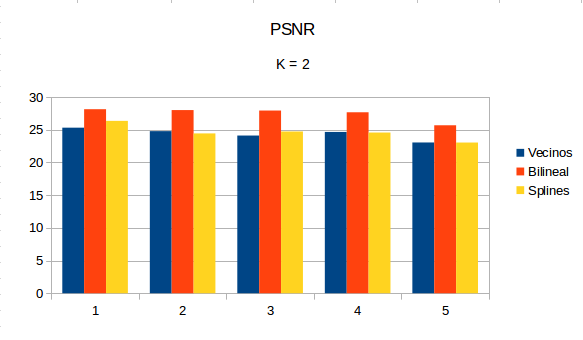
\includegraphics[scale=0.50]{imagenes/K2PSNR.png}
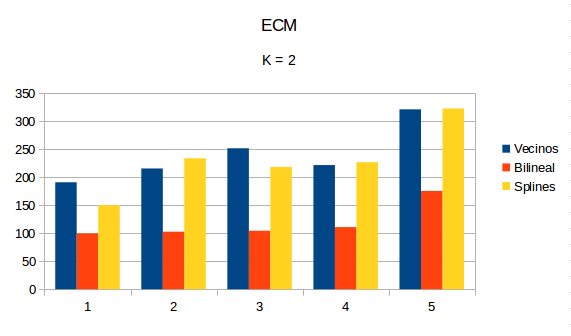
\includegraphics[scale=0.50]{imagenes/K2ECM.png}
\end{center}

\subsubsection{K = 4}
Para este segundo caso, es cierto que como esperabamos, el error cuadrático medio del método de los vecinos se dispara rápidamente mientras que los de interpolación bilineal y splines se mantienen prácticamente iguales. Lo mismo sucede para los valores de PSNR, siendo los del método de vecinos los únicos que disminuyen con una diferencia de casi 5 puntos.

\begin{center}
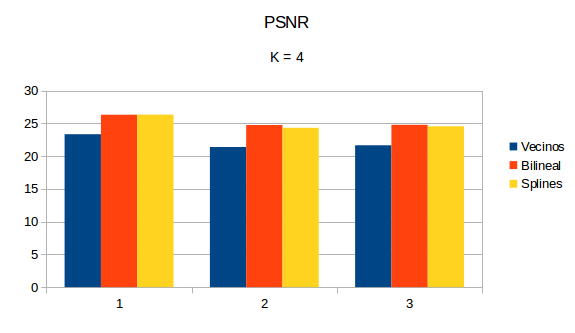
\includegraphics[scale=0.50]{imagenes/K4PSNR.png}
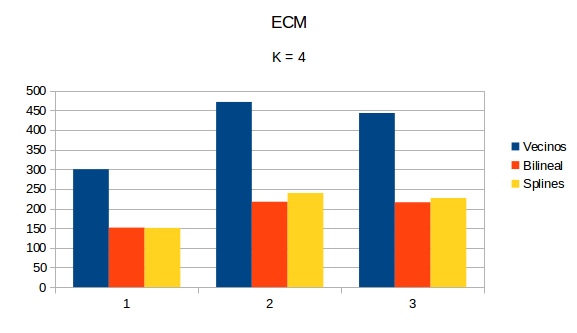
\includegraphics[scale=0.50]{imagenes/K4ECM.png}
\end{center}

\subsubsection{K = 6}
Entrando en valores de $k$ mucho más elevados, nuestro análisis empezó a dejar de coincidir con lo que creiamos en un primer momento serían los resultados finales, debido a que el método de Splines no logró sacar una diferencia notoria frente al de interpolación Bilineal, sino que incluso ambos métodos se mantuvieron prácticamente constantes.  Al momento de obtener los resultados nos llamaron poderosamente la atención los valores de ECM obtenidos para las tres primeras imágenes, pero luego de hacer un análisis en conjunto de estas, llegamos a la conclusión de que la suba desmesurada en estos valores se debe a la elevada variabilidad de los contrastes en la escena (el interior de un hogar muy decorado, la foto aérea de un barrio, etc). 

\begin{center}
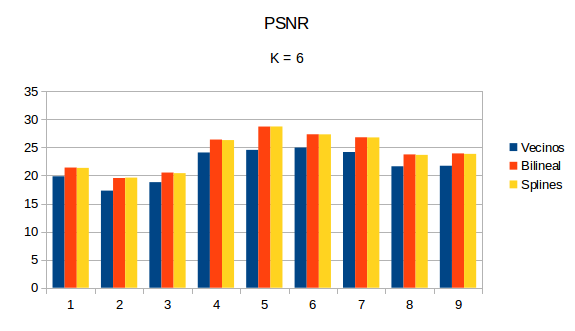
\includegraphics[scale=0.50]{imagenes/K6PSNR.png}
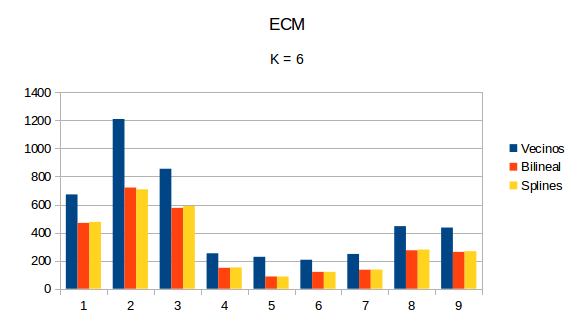
\includegraphics[scale=0.50]{imagenes/K6ECM.png}
\end{center}

\subsubsection{K = 10}
Por último, para valores que ya se consideran altos de $k$ el método de interpolación Bilineal todavía sigue desempeñandose igual o incluso a veces levemente mejor que el de Splines. Esto no solo contradice nuestra intuición, sino que debido a la performance de ambos, estos resultados colocan al método de interpolación como el más apto en relación benenficio/tiempo, muy por encima del de Splines (ambos ya muy por encima del método de vecinos a esta altura).

\begin{center}
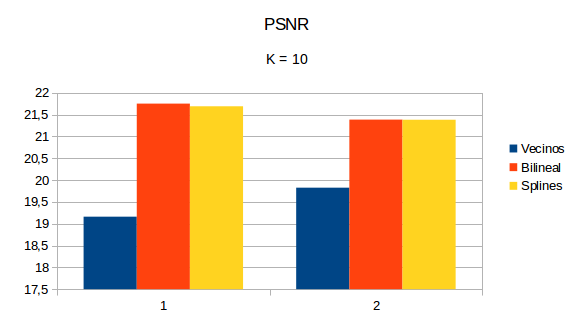
\includegraphics[scale=0.50]{imagenes/K10PSNR.png}
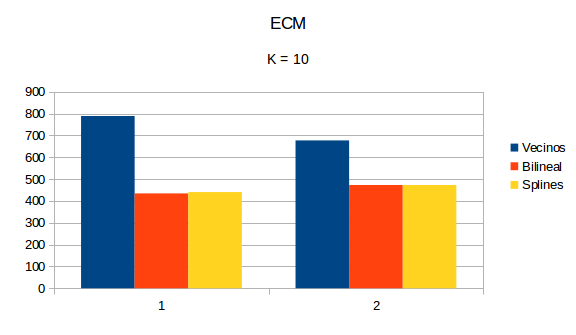
\includegraphics[scale=0.50]{imagenes/K10ECM.png}
\end{center}

\subsection{Análisis de tiempos}
El análisis de tiempo, a diferencia del de los métodos, no ofrecio ninguna respuesta que no hayamos podido intuir durante la codificación de los algoritmos. Es claro que a medida que el método se perfecciona en la búsqueda de resultados más suaves, también aumenta el tiempo necesario de cálculo.

\begin{center}
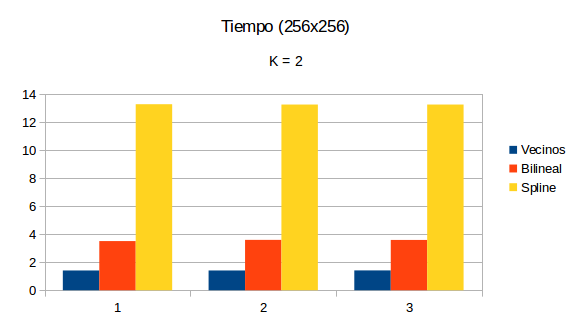
\includegraphics[scale=0.50]{imagenes/K2T1.png}
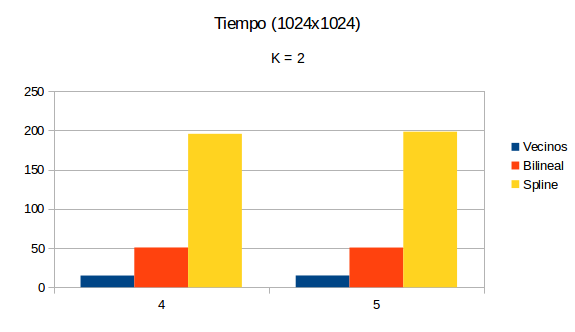
\includegraphics[scale=0.50]{imagenes/K2T2.png}
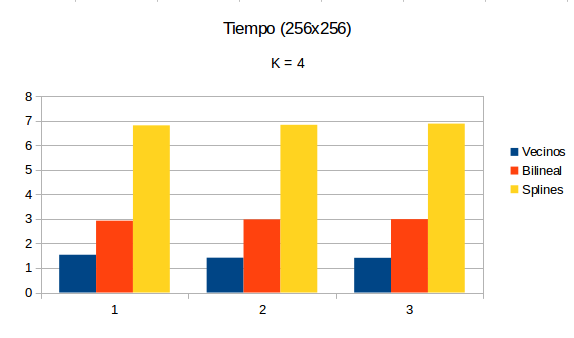
\includegraphics[scale=0.50]{imagenes/K4T.png}
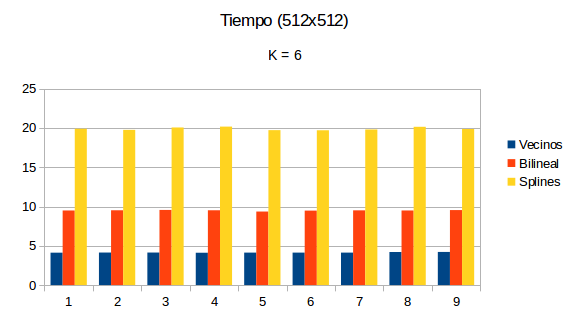
\includegraphics[scale=0.50]{imagenes/K6T.png}
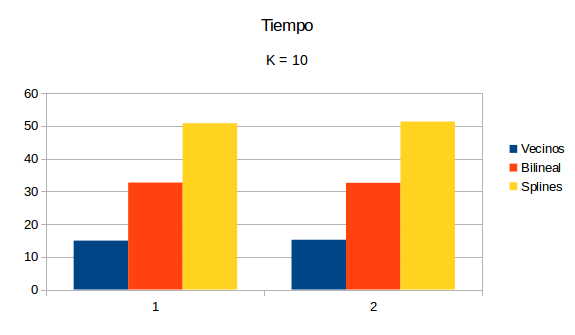
\includegraphics[scale=0.50]{imagenes/K10T.png}
\end{center}

